
This section applies the methods introduced in Section \ref{methodology} to both synthetic and
real‑world datasets and evaluates their capabilities in predictive accuracy, uncertainty calibration, and out-of-distribution (OOD) detection.

\subsection{Synthetic Dataset}
\label{exp:synthetic}
To evaluate MC-Dropout and SWAG for uncertainty quantification, experiments are conducted on a synthetic 
regression and binary classification task. Both tasks used a neural network with two fully-connected
hidden layers (32 neurons each with ReLU activations). For MC‑Dropout, dropout layers are added
after each hidden layer.

\paragraph{Regression Task}
A synthetic dataset is generated following:
\[
y = \sin(x) + 0.3\varepsilon, \quad \varepsilon \sim \mathcal{N}(0,1)
\]
Both models are trained on $x \in [-5, 5]$ and evaluated on $x \in [-8, 8]$.

\vspace{0.15cm}
As shown in Figure \ref{fig:regression}, both methods produce accurate mean predictions within the training region ($|x| \leq 5$), closely approximating $\sin(x)$. SWAG estimates thinner
uncertainty intervals than MC-Dropout, aligning with findings by \citet{maddox2019swag}.

Outside this region, the uncertainty bands increase as both methods detect OOD inputs. MC-Dropout
exhibits faster uncertainty growth, with uncertainty intervals widening more rapidly than SWAG beyond
$|x| > 5$. SWAG maintains tighter confidence bands while still showing some uncertainty expansion.

The sample points form vertical patterns ("pillars") in both cases. These result from 200 stochastic
predictions being sampled at each of the 100 equidistant test points along the x-axis. For MC-Dropout,
predictions come from different thinned subnetworks, while for SWAG they derive from weight samples
$\mathbf{w}^{(s)} \sim q_{\mathrm{SWAG}}$.

SWAG's samples follow a certain structure, where connecting e.g. the maximum prediction at each test
point will form a smooth curve. This is because these samples come from the same set of weights,
i.e. the same model. MC-Dropout's more irregular dispersion reflects the random neuron deactivations
from different dropout masks \citep{gal2016mcdropout}.

\vspace{0.15cm}
These observations align with theoretical expectations, MC-Dropout's sampling produces noisier but more
conservative uncertainty estimates \citep{gal2016mcdropout}, while SWAG's weight-space sampling provides
a geometrically structured uncertainty quantification. Both methods distinguish between in-domain
confidence and out-of-domain uncertainty.

\FloatBarrier

\begin{figure}[ht]
  \centering
  \begin{subfigure}{0.8\textwidth}
    \centering
    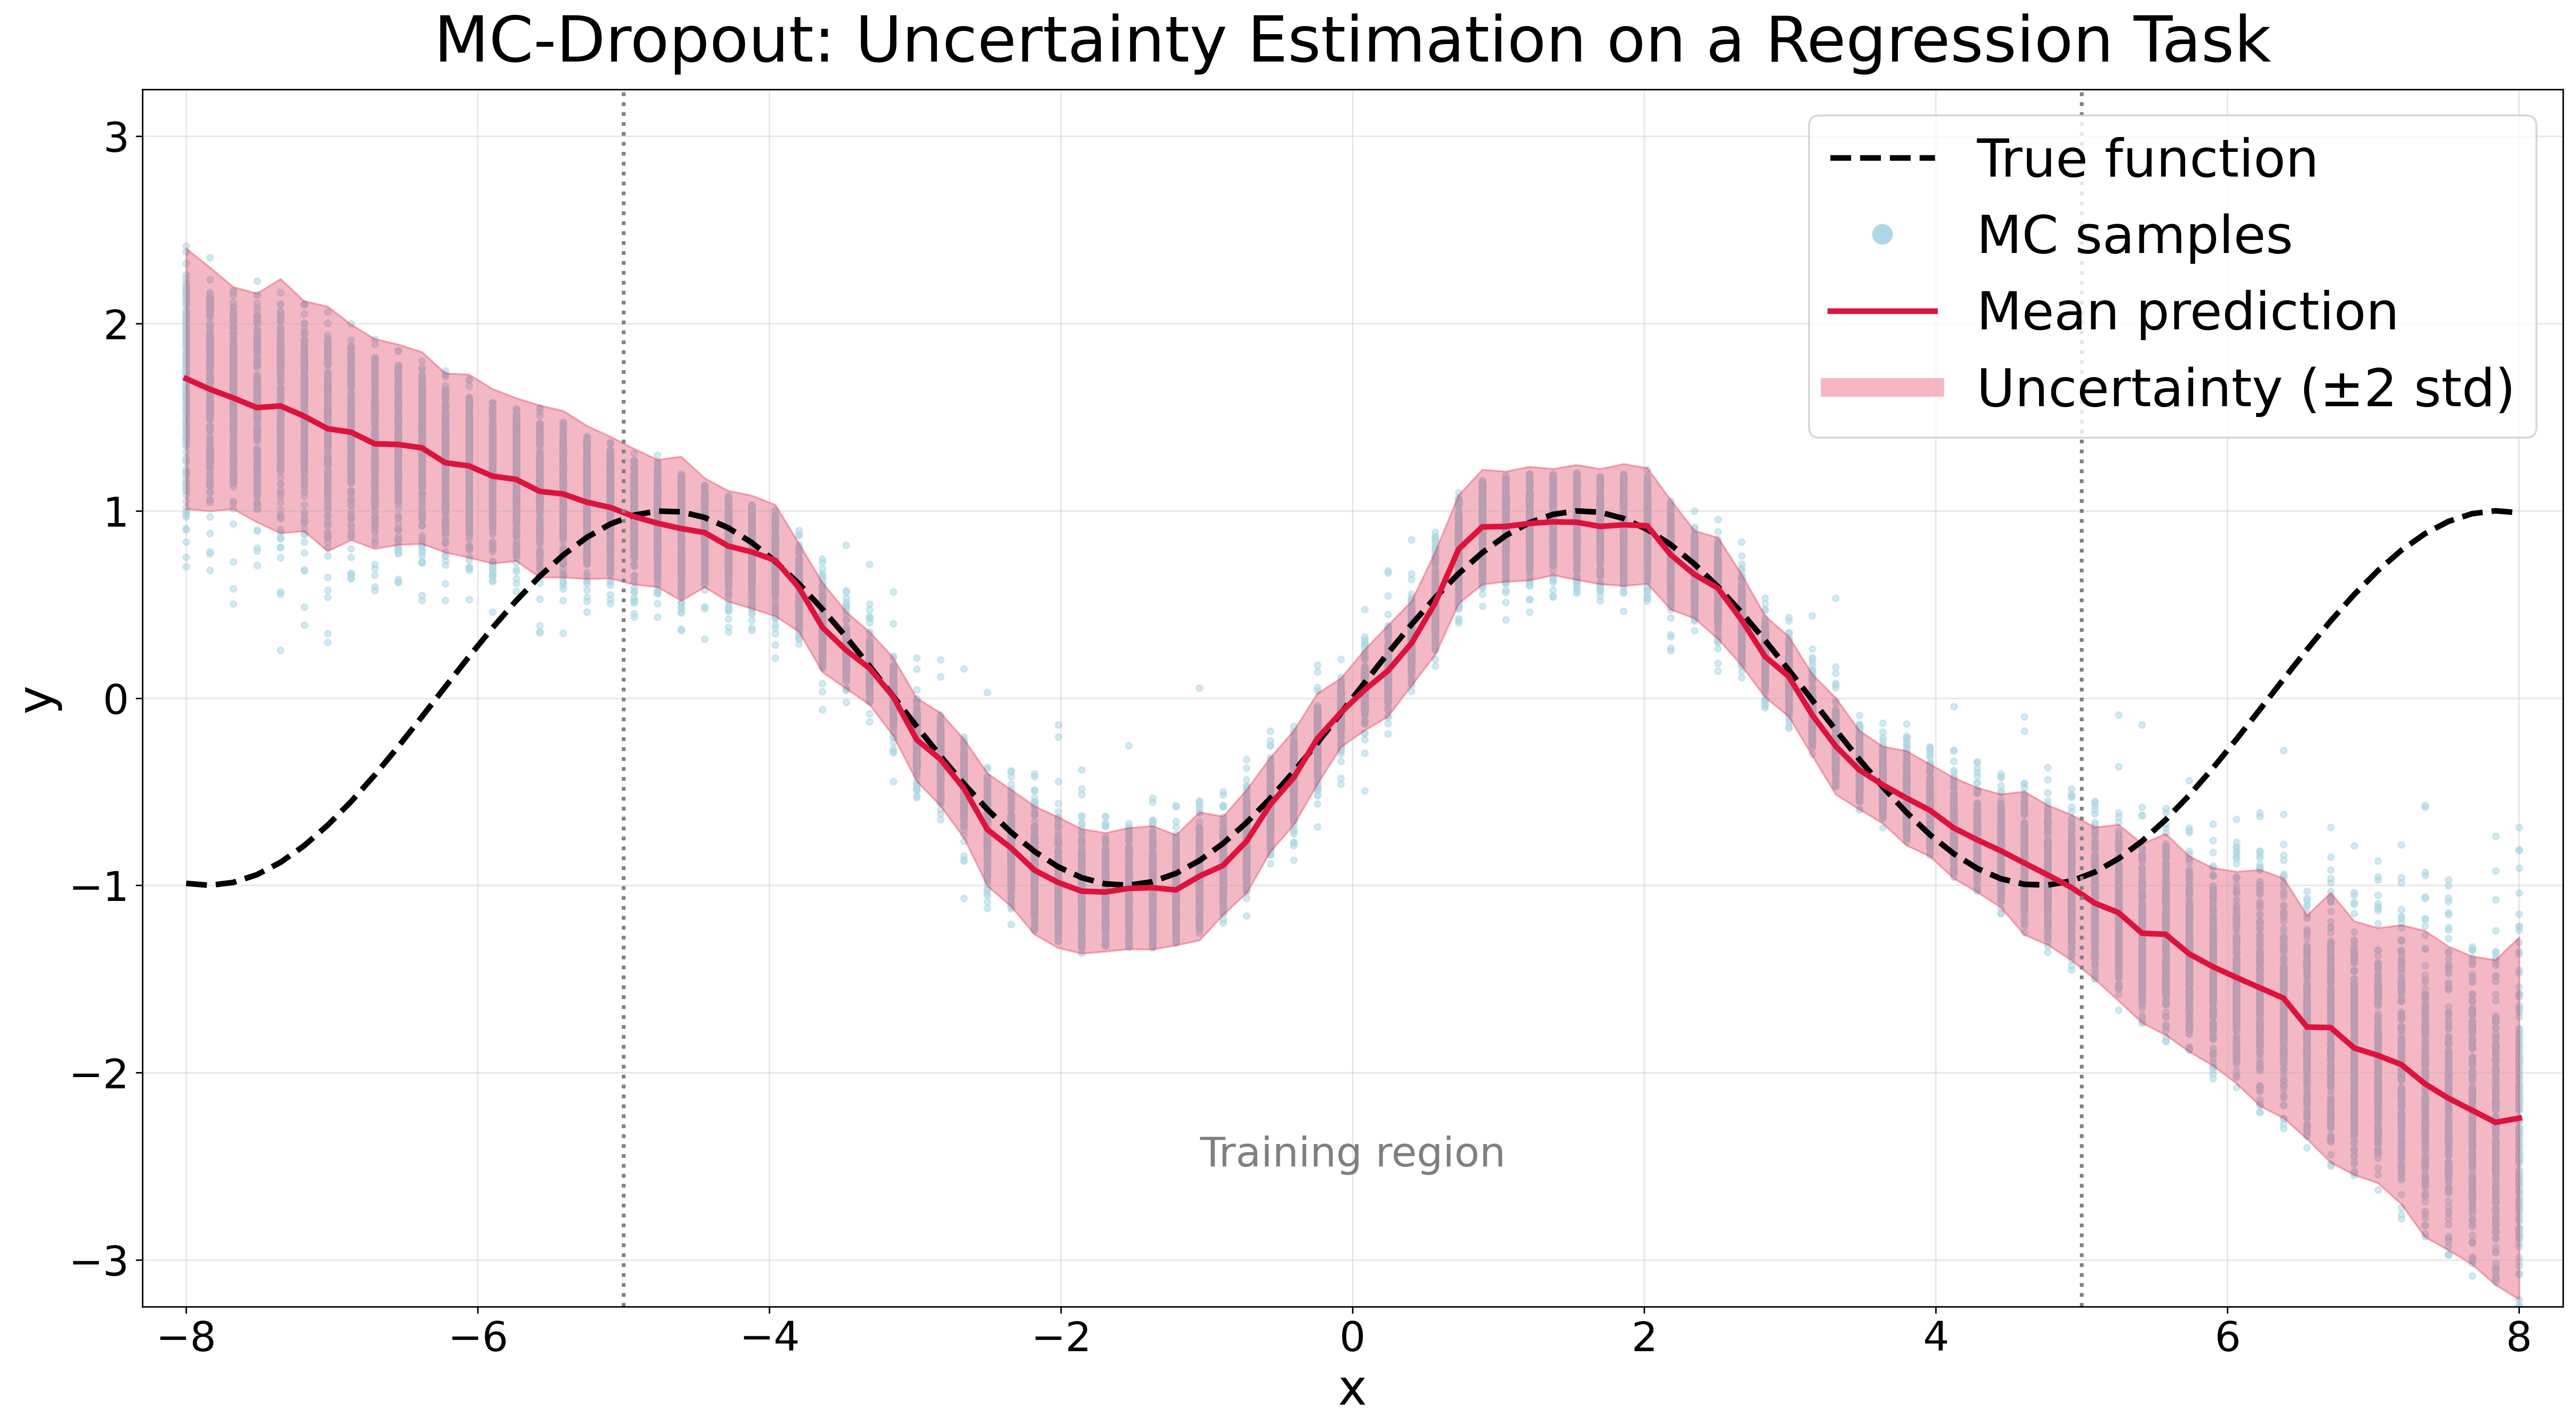
\includegraphics[width=\textwidth]{plots/mcd_regression.png}
  \end{subfigure}
  
  \vspace{0.3cm}
  \begin{subfigure}{0.8\textwidth}
    \centering
    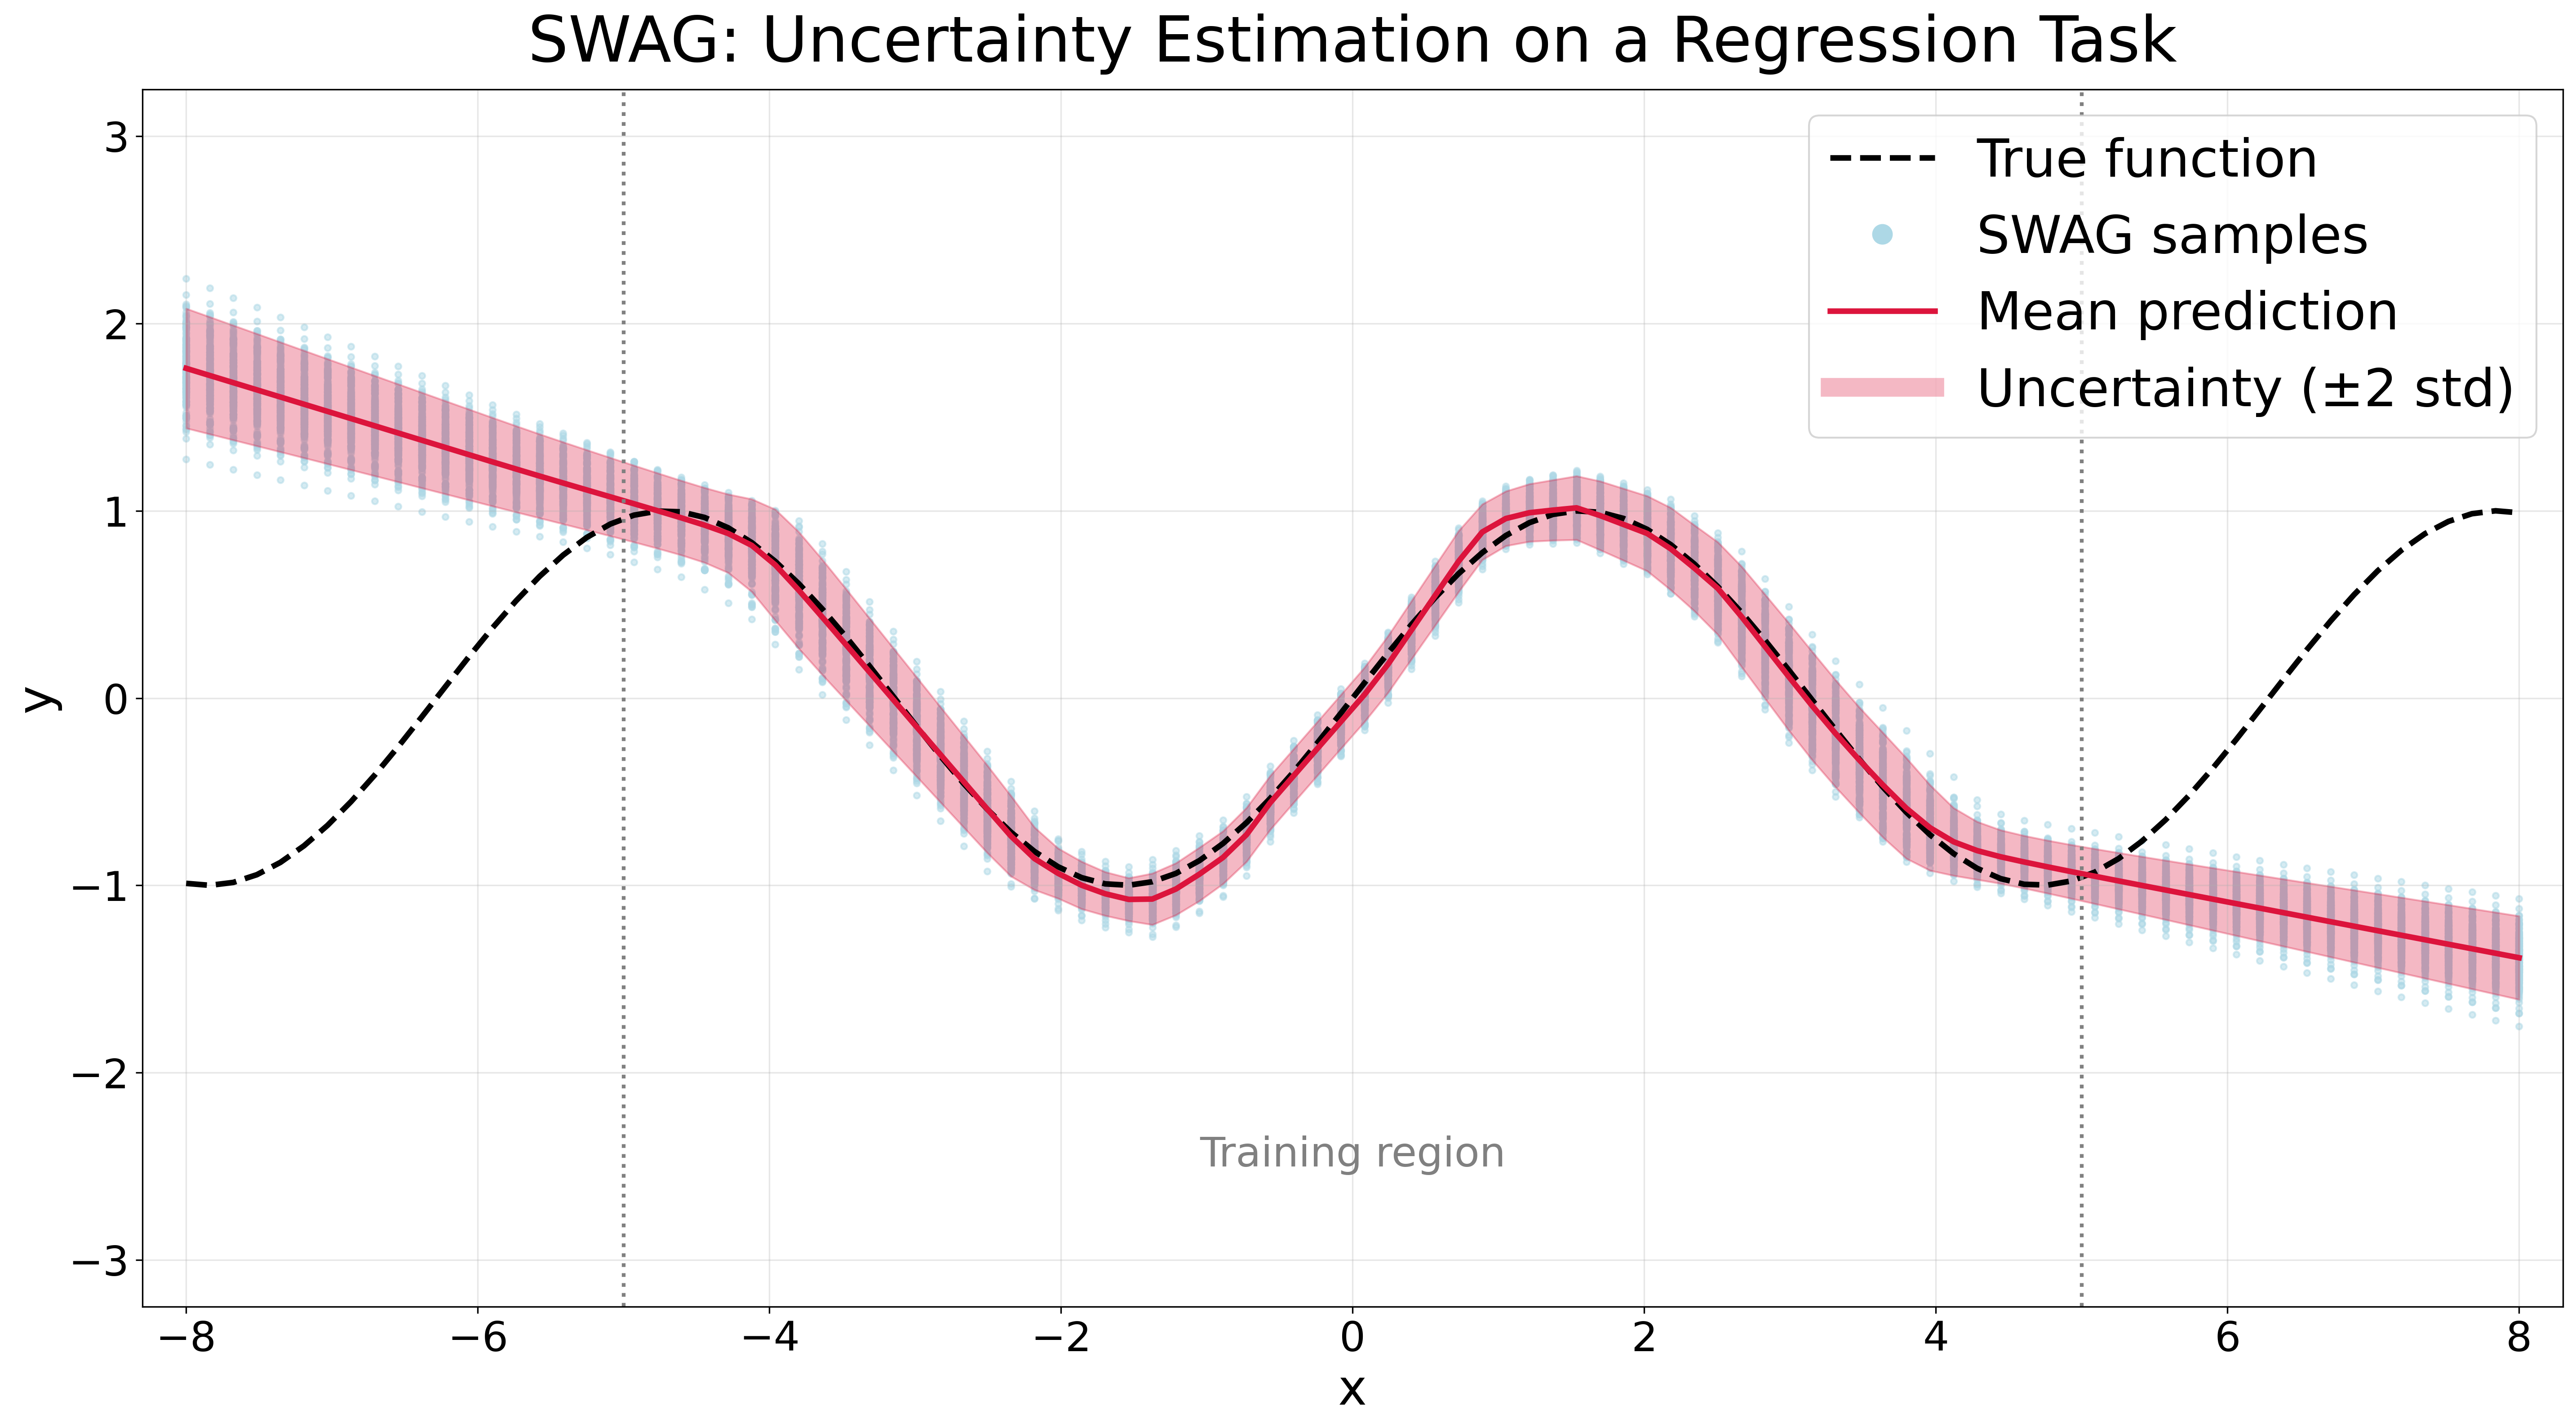
\includegraphics[width=\textwidth]{plots/swag_regression.png}
  \end{subfigure}
  \caption{Regression uncertainty estimation: MC-Dropout (top) and SWAG (bottom). Training domain ($|x| \leq 5$) marked by dashed lines.}
  \label{fig:regression}
\end{figure}

\FloatBarrier

\newpage
\paragraph{Classification Task}
The binary classification task uses a "two moons" dataset generated with scikit-learn \citep{scikit-learn}, it contains 500 training points with a nonlinear class boundary.

\vspace{0.15cm}
Figure \ref{fig:classification} shows both methods assign low uncertainty near training data, with sharp
decision boundaries (zone where the model transitions from predicting one class to the other). Both
increase predictive uncertainty in regions far from training data, successfully identifying OOD areas.
SWAG provides a smoother uncertainty estimation, while MC-Dropout produces a more scattered predictive
uncertainty, especially in the extrapolation region. 

Notably, some noisy points located in the wrong class' region (at approximately $(1.5, -0.5)$ and
$(0.5, 0.5)$) induce uncertainty spikes in SWAG but not MC-Dropout. This demonstrates SWAG's sensitivity
to weight-space perturbations \citep{izmailov2019swa}, as its covariance propagates uncertainty from
anomalies to neighboring regions. Near these noisy points, SWAG shows broader uncertainty intervals
while maintaining thinner boundaries elsewhere (e.g., near $(0,0)$).

\FloatBarrier

\begin{figure}[ht]
  \centering
  \begin{subfigure}{0.8\textwidth}
    \centering
    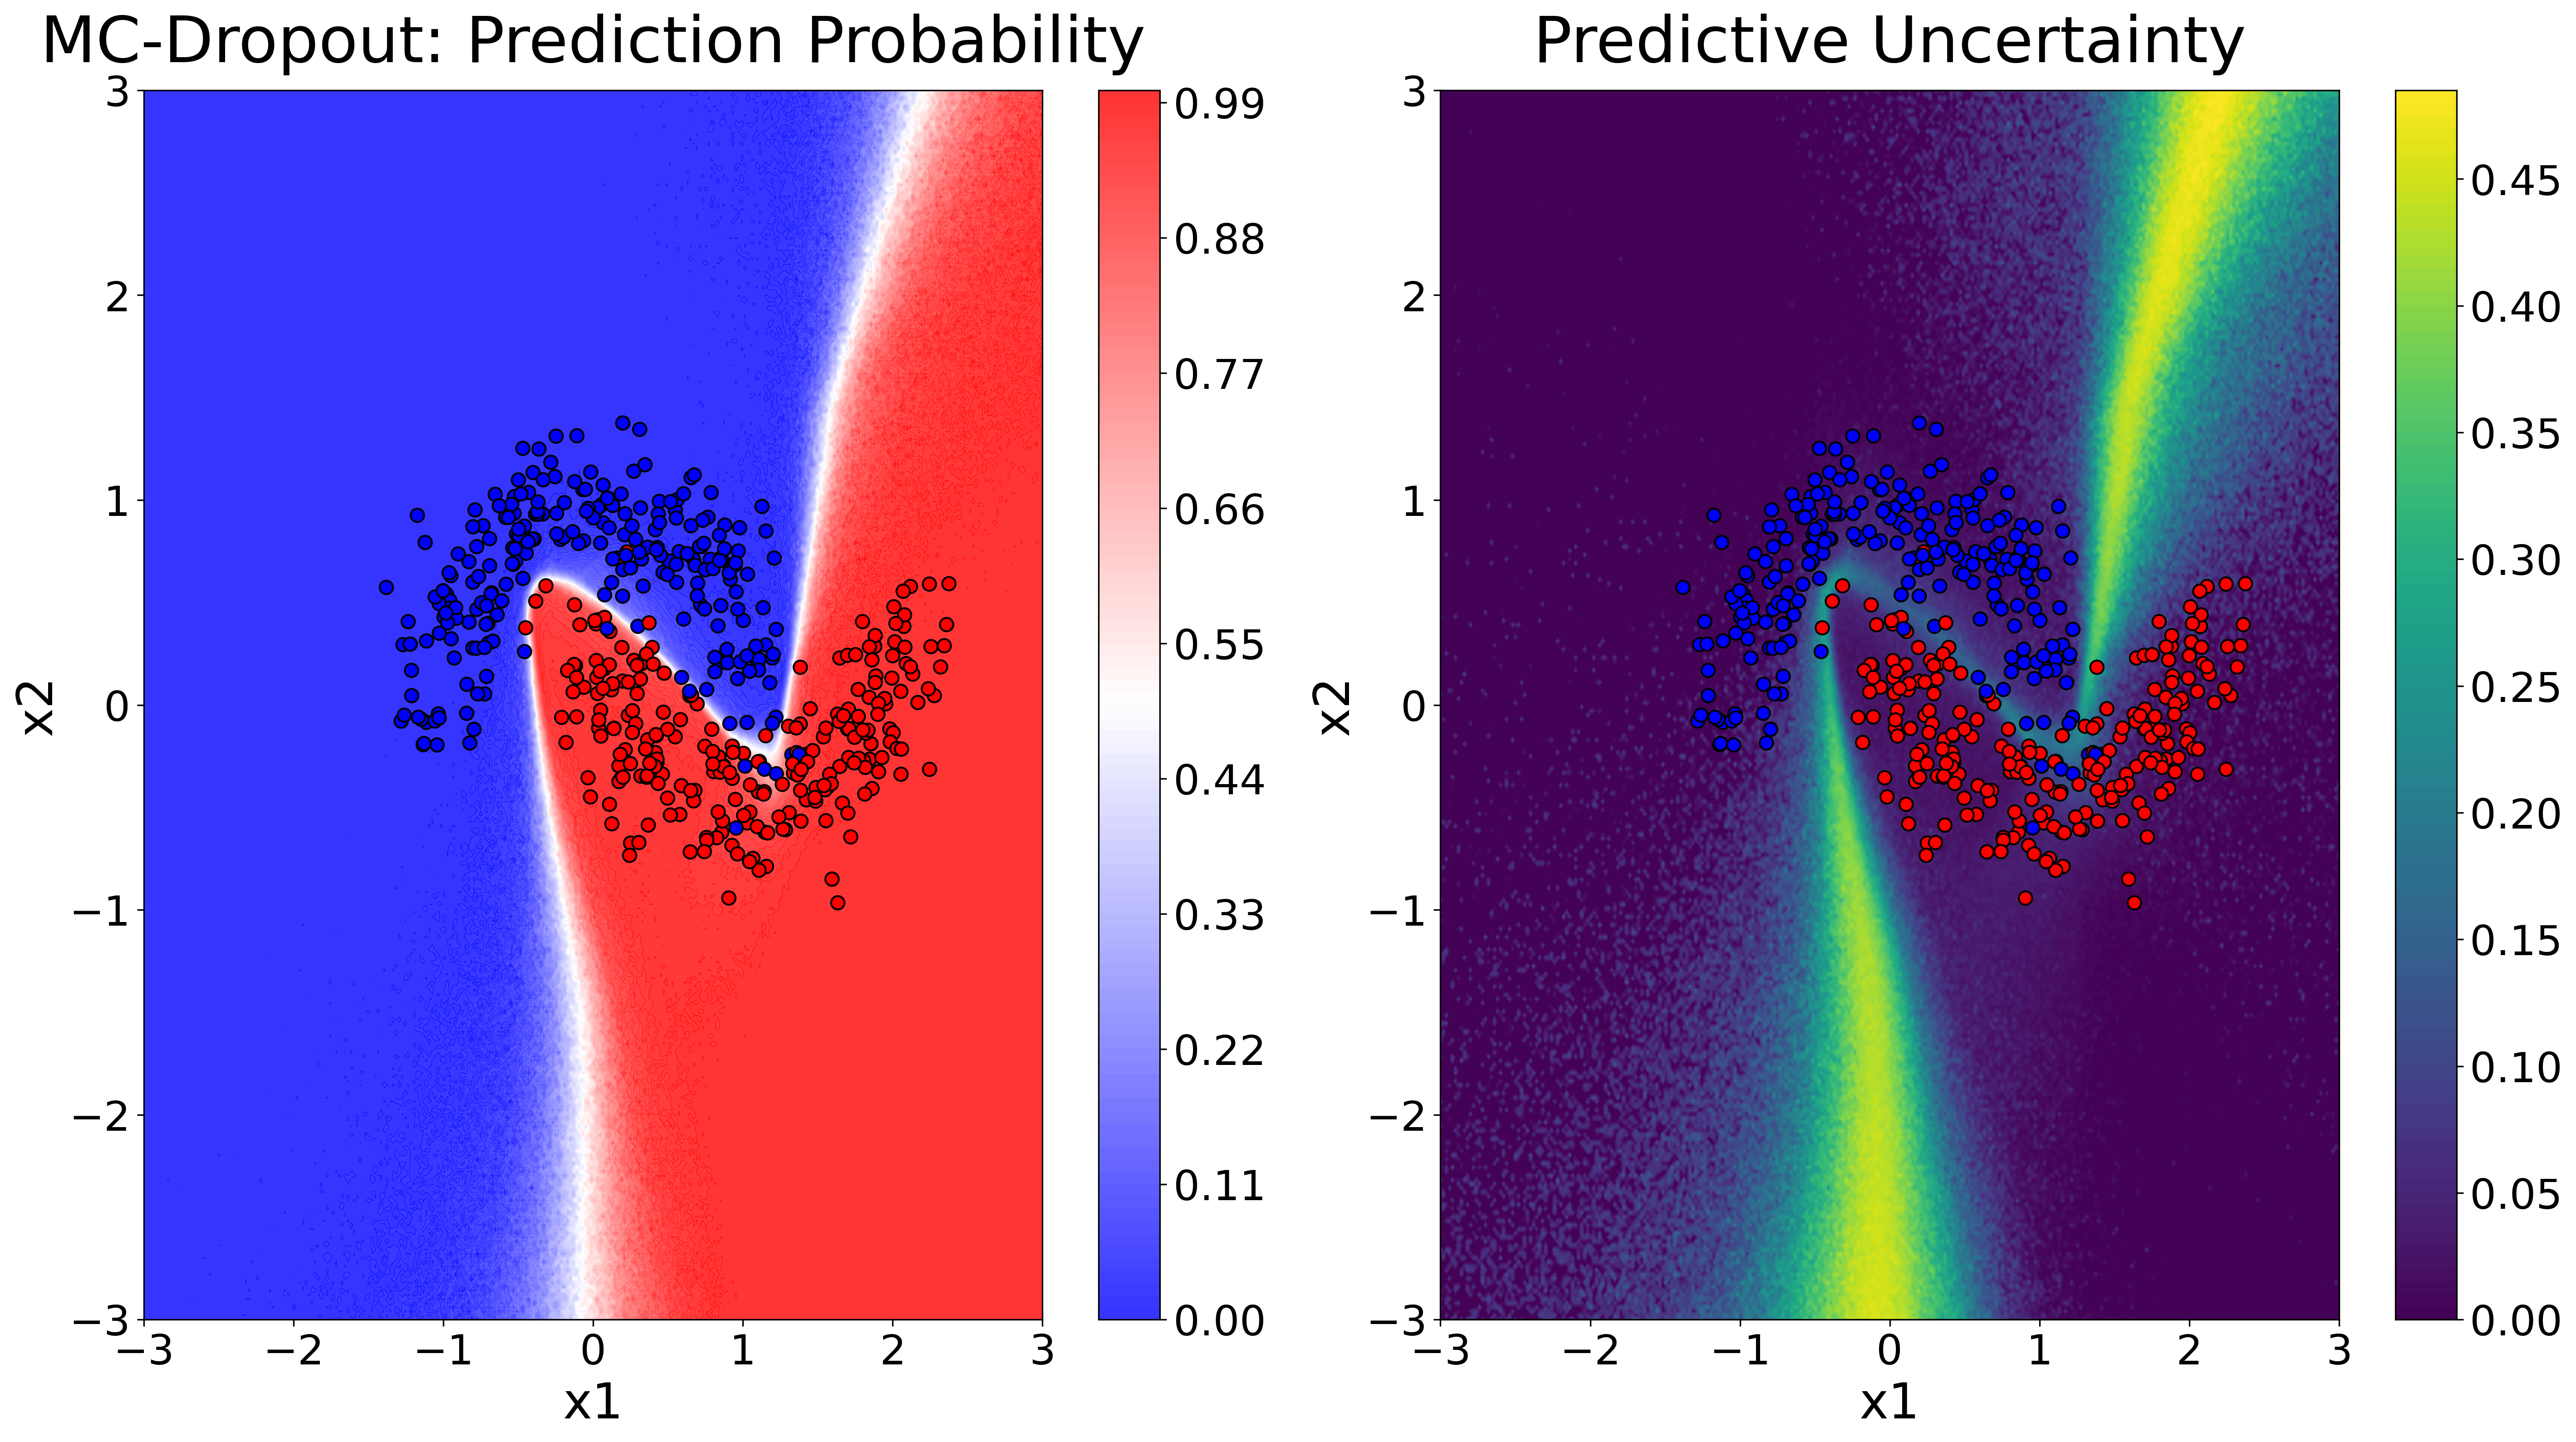
\includegraphics[width=\textwidth]{plots/mcd_classification.png}
  \end{subfigure}
  
  \vspace{0.3cm}
  \begin{subfigure}{0.8\textwidth}
    \centering
    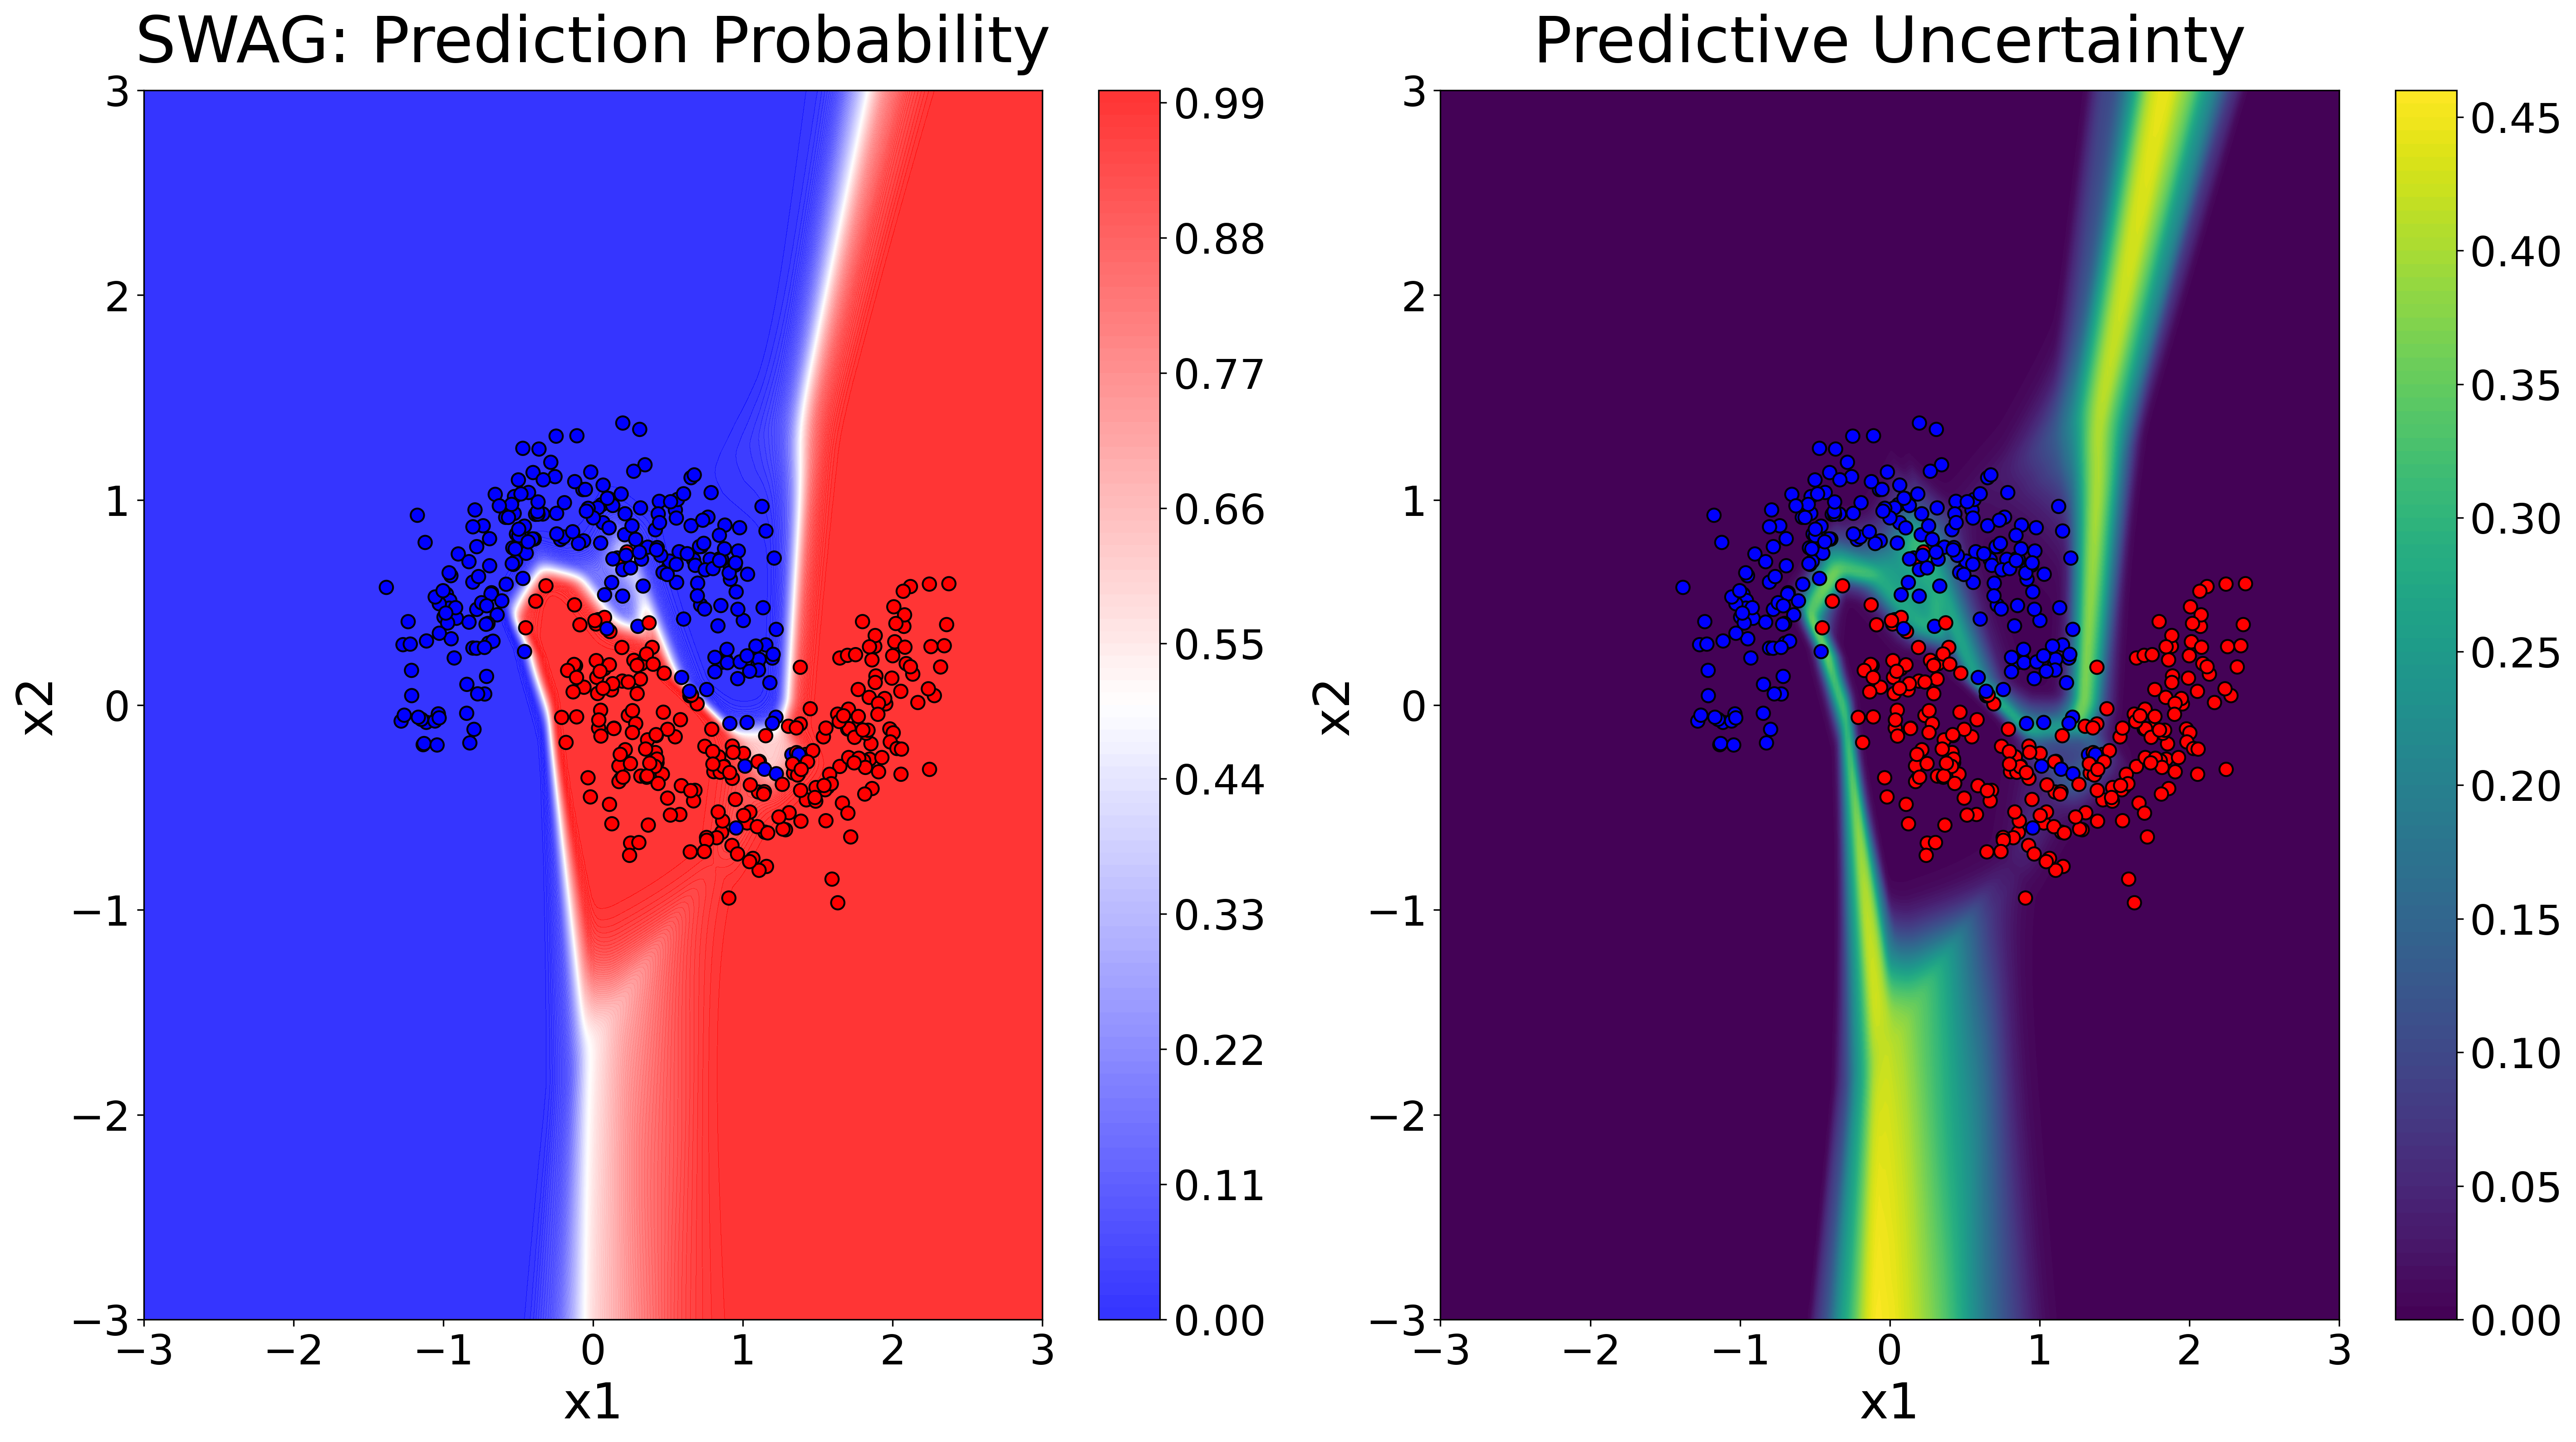
\includegraphics[width=\textwidth]{plots/swag_classification.png}
  \end{subfigure}
  \caption{Classification uncertainty: MC-Dropout (top) and SWAG (bottom). Color indicates true class (red/blue).}
  \label{fig:classification}
\end{figure}

\FloatBarrier



\newpage
\subsection{Evaluation on Real-world Data}
\label{exp:real-world_data}
To assess practical performance, the Boston Housing dataset is used \citep{harrison1978bh}.
It consists of 506 observations of housing prices in Boston suburbs. The response variable is the median
home value (in \$1000s), with features including crime rate, average rooms and highway accessibility.
Following ethical research standards, the racially problematic \texttt{B} variable is excluded.
It encoded the proportion of Black residents and reflected discriminatory assumptions in its original
formulation \citep[see, e.g.,][]{carlisle2020bh_ethicalIssue}.

\paragraph{Model Architecture and Training}
A neural network with four fully connected hidden layers is trained to predict standardized housing
prices. Hyperparameter tuning is conducted using a randomized grid search on a previously unseen
validation set. For MC-Dropout, dropout layers are once again added after each hidden layer.
Both models are trained using the Adam optimizer with a tuned learning rate and weight decay.

Table \ref{tab:bh_metrics} summarizes the evaluation results on the test set using three key metrics:
Root Mean Squared Error (RMSE) measures predictive accuracy (lower values preferred), Negative
Log-Likelihood (NLL) assesses uncertainty calibration (lower values indicate better calibration) and
Prediction Interval Coverage Probability (PICP) evaluates the reliability of 95\,\% uncertainty
intervals (values closer to 95\,\% reflect superior uncertainty estimation).

\begin{table}[h!]
\centering
\begin{tabular}{lccc}
\toprule
Method & RMSE & NLL & PICP (95\,\%) \\
\midrule
MC-Dropout & 0.4033 & 0.6814 & 0.7352 \\
SWAG       & 0.3947 & 0.2218 & 0.9314 \\
\bottomrule
\end{tabular}
\caption{Test performance on the Boston Housing dataset.}
\label{tab:bh_metrics}
\end{table}

Both methods achieve comparable point-prediction accuracy, as evidenced by their similar RMSE values.
However, SWAG demonstrates significantly better uncertainty calibration, with a much lower NLL and a
near-ideal PICP of 93.14\,\%. MC-Dropout's PICP of 73.52\,\% indicates systematic undercoverage.
The notable discrepancy in NLL values further reveals MC-Dropout's tendency toward overconfidence,
as it frequently assigns high certainty to incorrect predictions.


\paragraph{Uncertainty Behavior Analysis}
Figure \ref{fig:bh_uncertainty_comp2x2} provides a comparative analysis of uncertainty characteristics between MC-Dropout and SWAG.

The top-left subplot displays histograms of predictive standard deviations, revealing distinct
distributional profiles. MC-Dropout exhibits a sharp peak near 0.16, indicating overconfident estimates
with limited variability, whereas SWAG generates a broader distribution centered near 0.2 with an
extended right tail, reflecting more moderate and diverse uncertainty quantification.

In the top-right scatter plot of absolute residuals versus predictive standard deviations, SWAG displays a
wider vertical spread of points, suggesting that it assigns greater uncertainty to predictions with larger
errors. On the other hand, MC-Dropout's points are more tightly clustered near the origin, indicating
uniformly low uncertainty estimates even when residuals are non-negligible. This pattern reinforces the
impression of overconfidence in MC-Dropout's uncertainty outputs.

The bottom row consists of two calibration plots, where predicted means are plotted against true target
values and shaded confidence bands represent 95\,\% predictive intervals. While both models align well
along the identity line in high-density regions, SWAG produces slightly wider confidence bands. This
demonstrates more conservative and better-calibrated uncertainty estimates.

\FloatBarrier

\begin{figure}[ht]
    \centering
    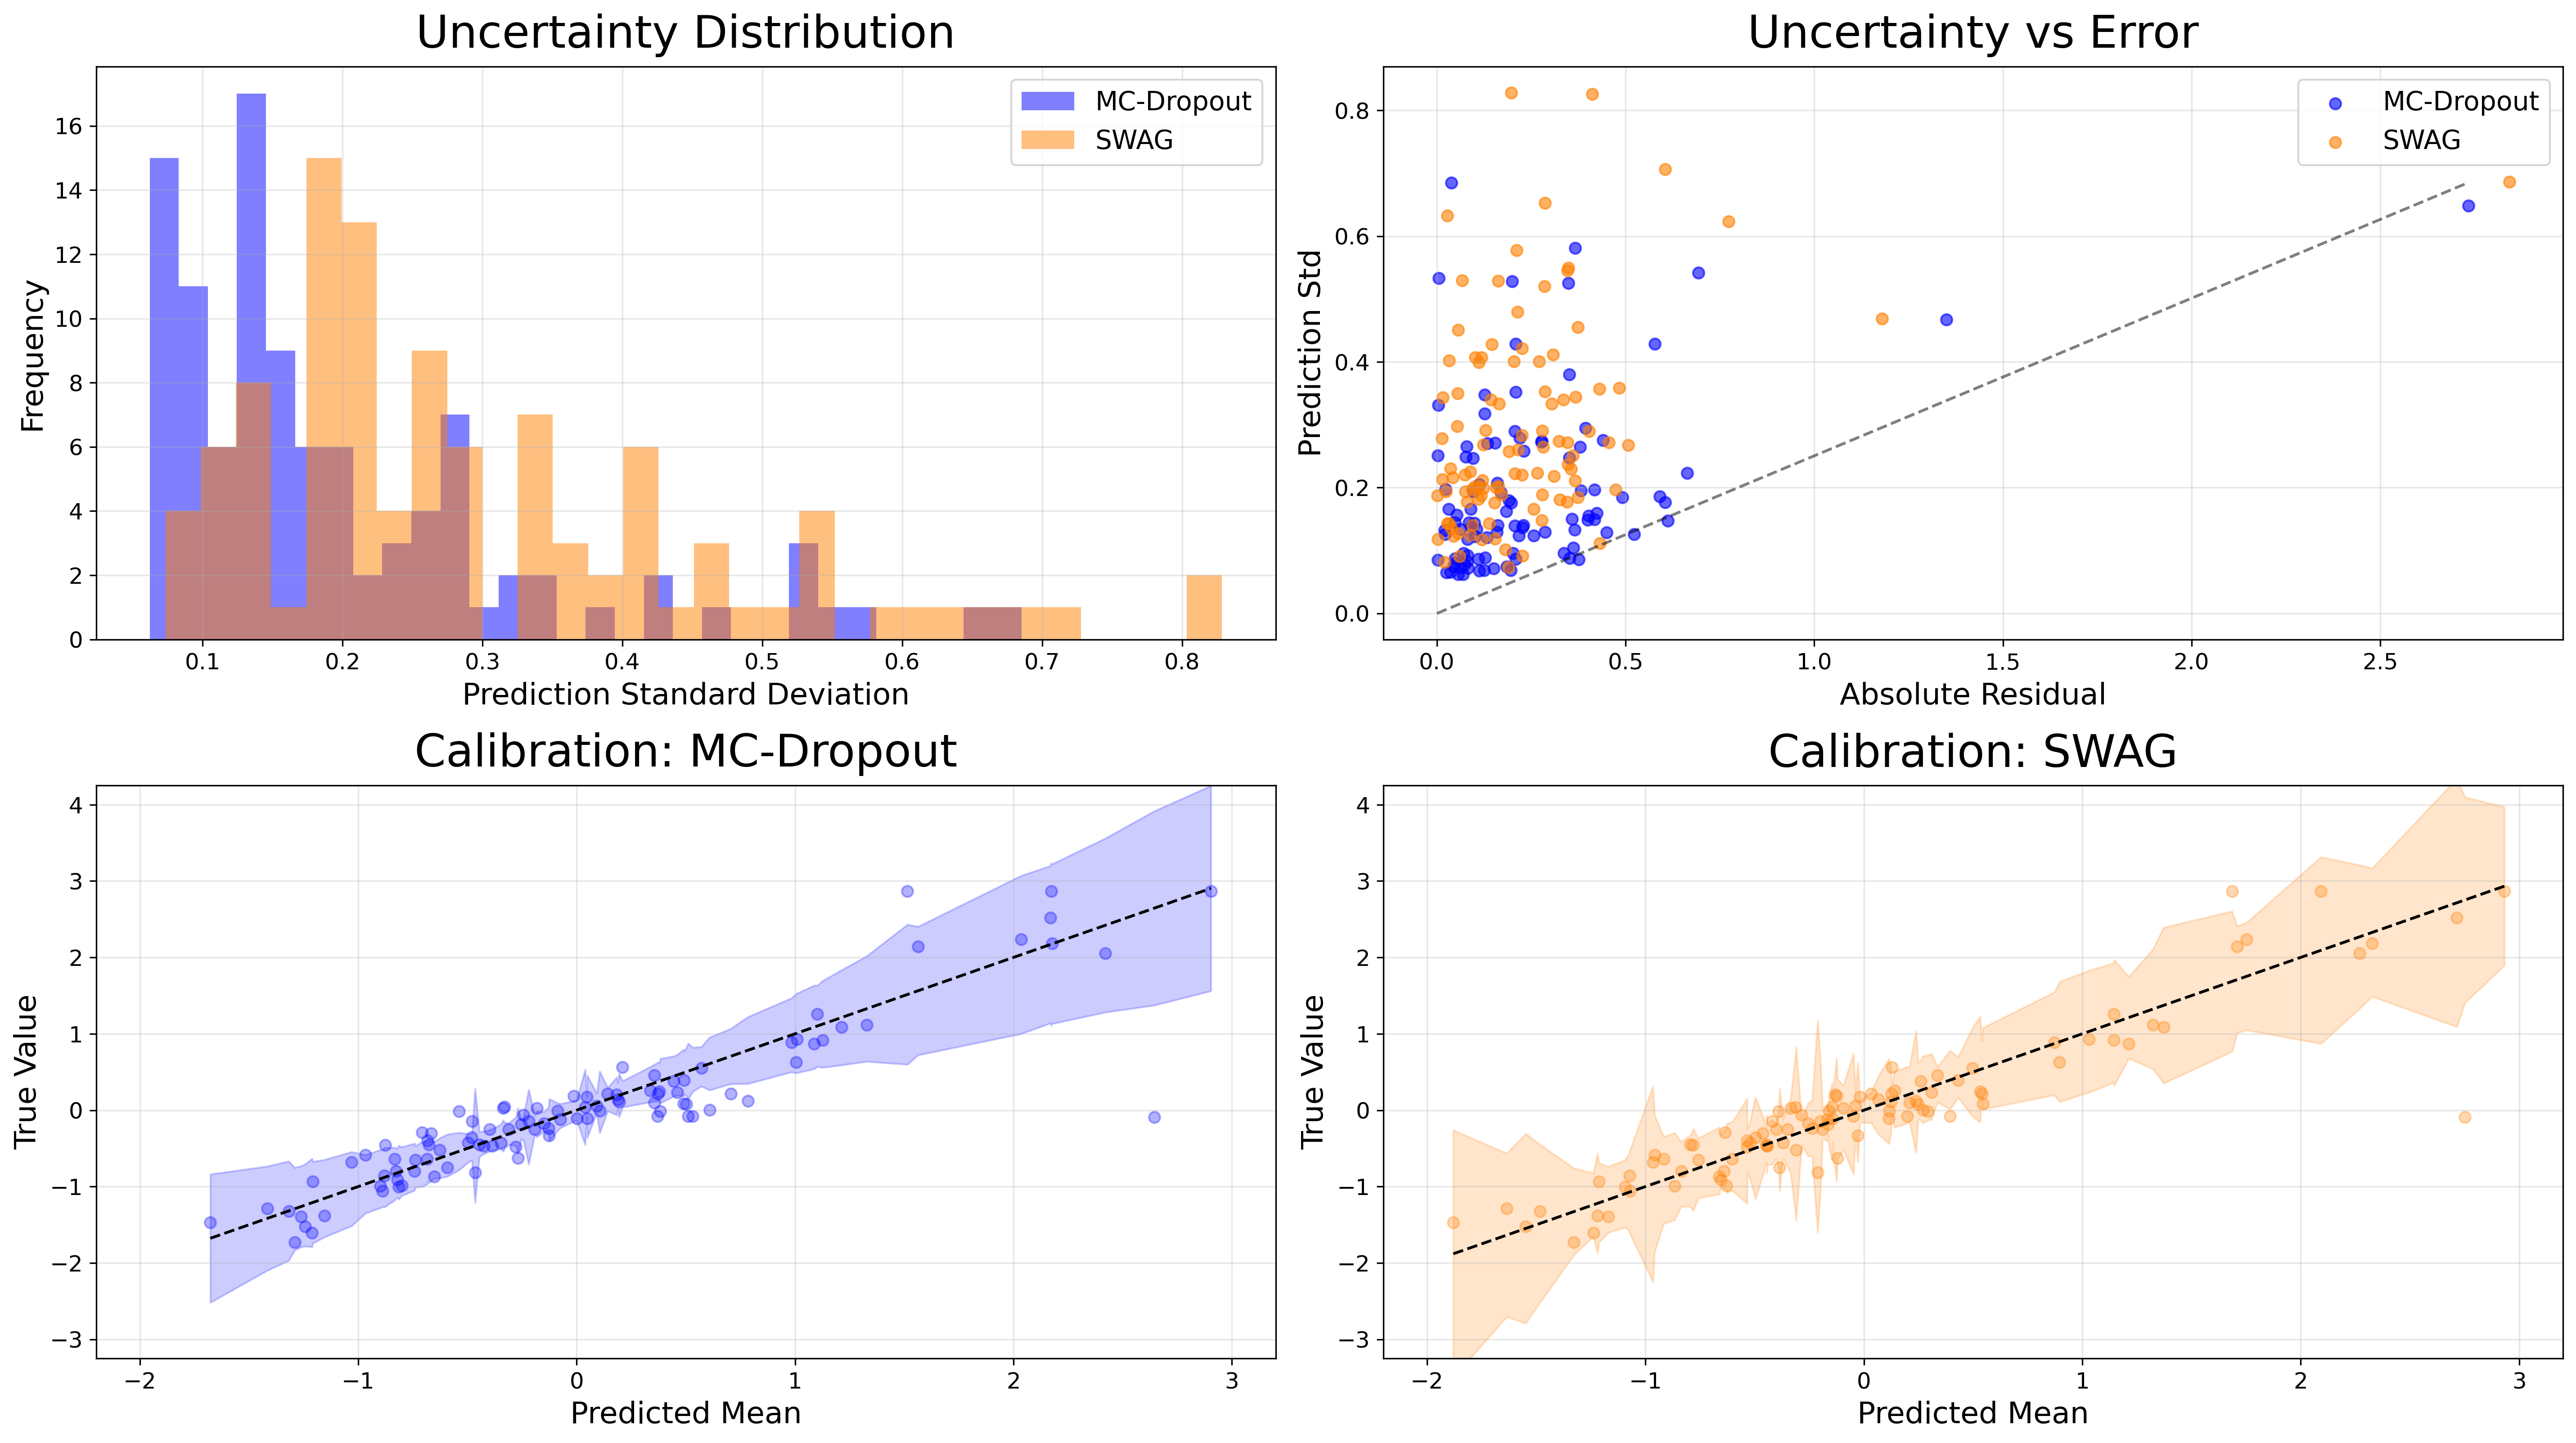
\includegraphics[width=0.9\linewidth]{plots/bh_uncertainty_comp2x2.png}
    \caption{Comparison of uncertainty behaviors for MC-Dropout and SWAG on the Boston Housing dataset.}
    \label{fig:bh_uncertainty_comp2x2}
\end{figure}

\FloatBarrier


\paragraph{Out-of-Distribution Analysis}
To evaluate the robustness of uncertainty estimation under distribution shift, two types of
out-of-distribution (OOD) scenarios are examined. Natural OOD samples with exceptionally high median
income (\texttt{MedInc}) and artificially perturbed samples with amplified income and reduced occupancy.
Table~\ref{tab:ood_results} displays predictive accuracy (RMSE) and uncertainty calibration (NLL) across
in-domain and OOD conditions.

\begin{table}[h!]
\centering
\begin{tabular}{lccccc}
\toprule
 & \multicolumn{2}{c}{MC-Dropout} & \multicolumn{2}{c}{SWAG} \\
Scenario & RMSE & NLL & RMSE & NLL \\
\midrule
In-domain & 0.4033 & 0.6814 & 0.3947 & 0.2218 \\
Natural OOD & 0.2768 & 0.2331 & 0.3838 & 0.6708 \\
Artificial OOD & 0.4283 & 0.7249 & 0.4094 & 0.3006 \\
\bottomrule
\end{tabular}
\caption{OOD performance comparison.}
\label{tab:ood_results}
\end{table}

For natural OOD samples, MC-Dropout shows point-prediction accuracy with the RMSE decreasing from 0.4033 to
0.2768, but exhibits a substantial NLL reduction (0.6814 to 0.2331). This divergence suggests potentially
overconfident uncertainty estimates that fail to properly reflect distribution shift. In contrast, SWAG
maintains stable predictive accuracy (RMSE: 0.3947 to 0.3838) while appropriately increasing NLL (0.2218
to 0.6708), indicating more cautious uncertainty estimation under distribution shift.

In the artificial OOD scenario, both methods show degraded performance. MC-Dropout's RMSE increases to
0.4283 and NLL to 0.7249, while SWAG's RMSE increases to 0.4094 and NLL to 0.3006. The increased NLL
indicates worse uncertainty calibration compared to in-domain samples and SWAG maintains its superior
calibration. Both methods show a very similar relative response under artificial perturbations.

Figure \ref{fig:bh_ood_comp} complements the tabular metrics by visualizing the distribution of predictive
standard deviations (i.e., uncertainty) shifts between in-domain and artificial OOD conditions. For MC-Dropout (left panel), the histogram shows negligible distributional change with marginally
increased maximum uncertainty, indicating limited responsiveness to distribution shift. SWAG (right panel)
displays a substantial increase in maximum uncertainty (33\,\%), this demonstrates that SWAG has the
capacity to effectively register distributional changes and inflate uncertainty accordingly
\citep{maddox2019swag}.

\FloatBarrier

\begin{figure}[ht]
    \centering
    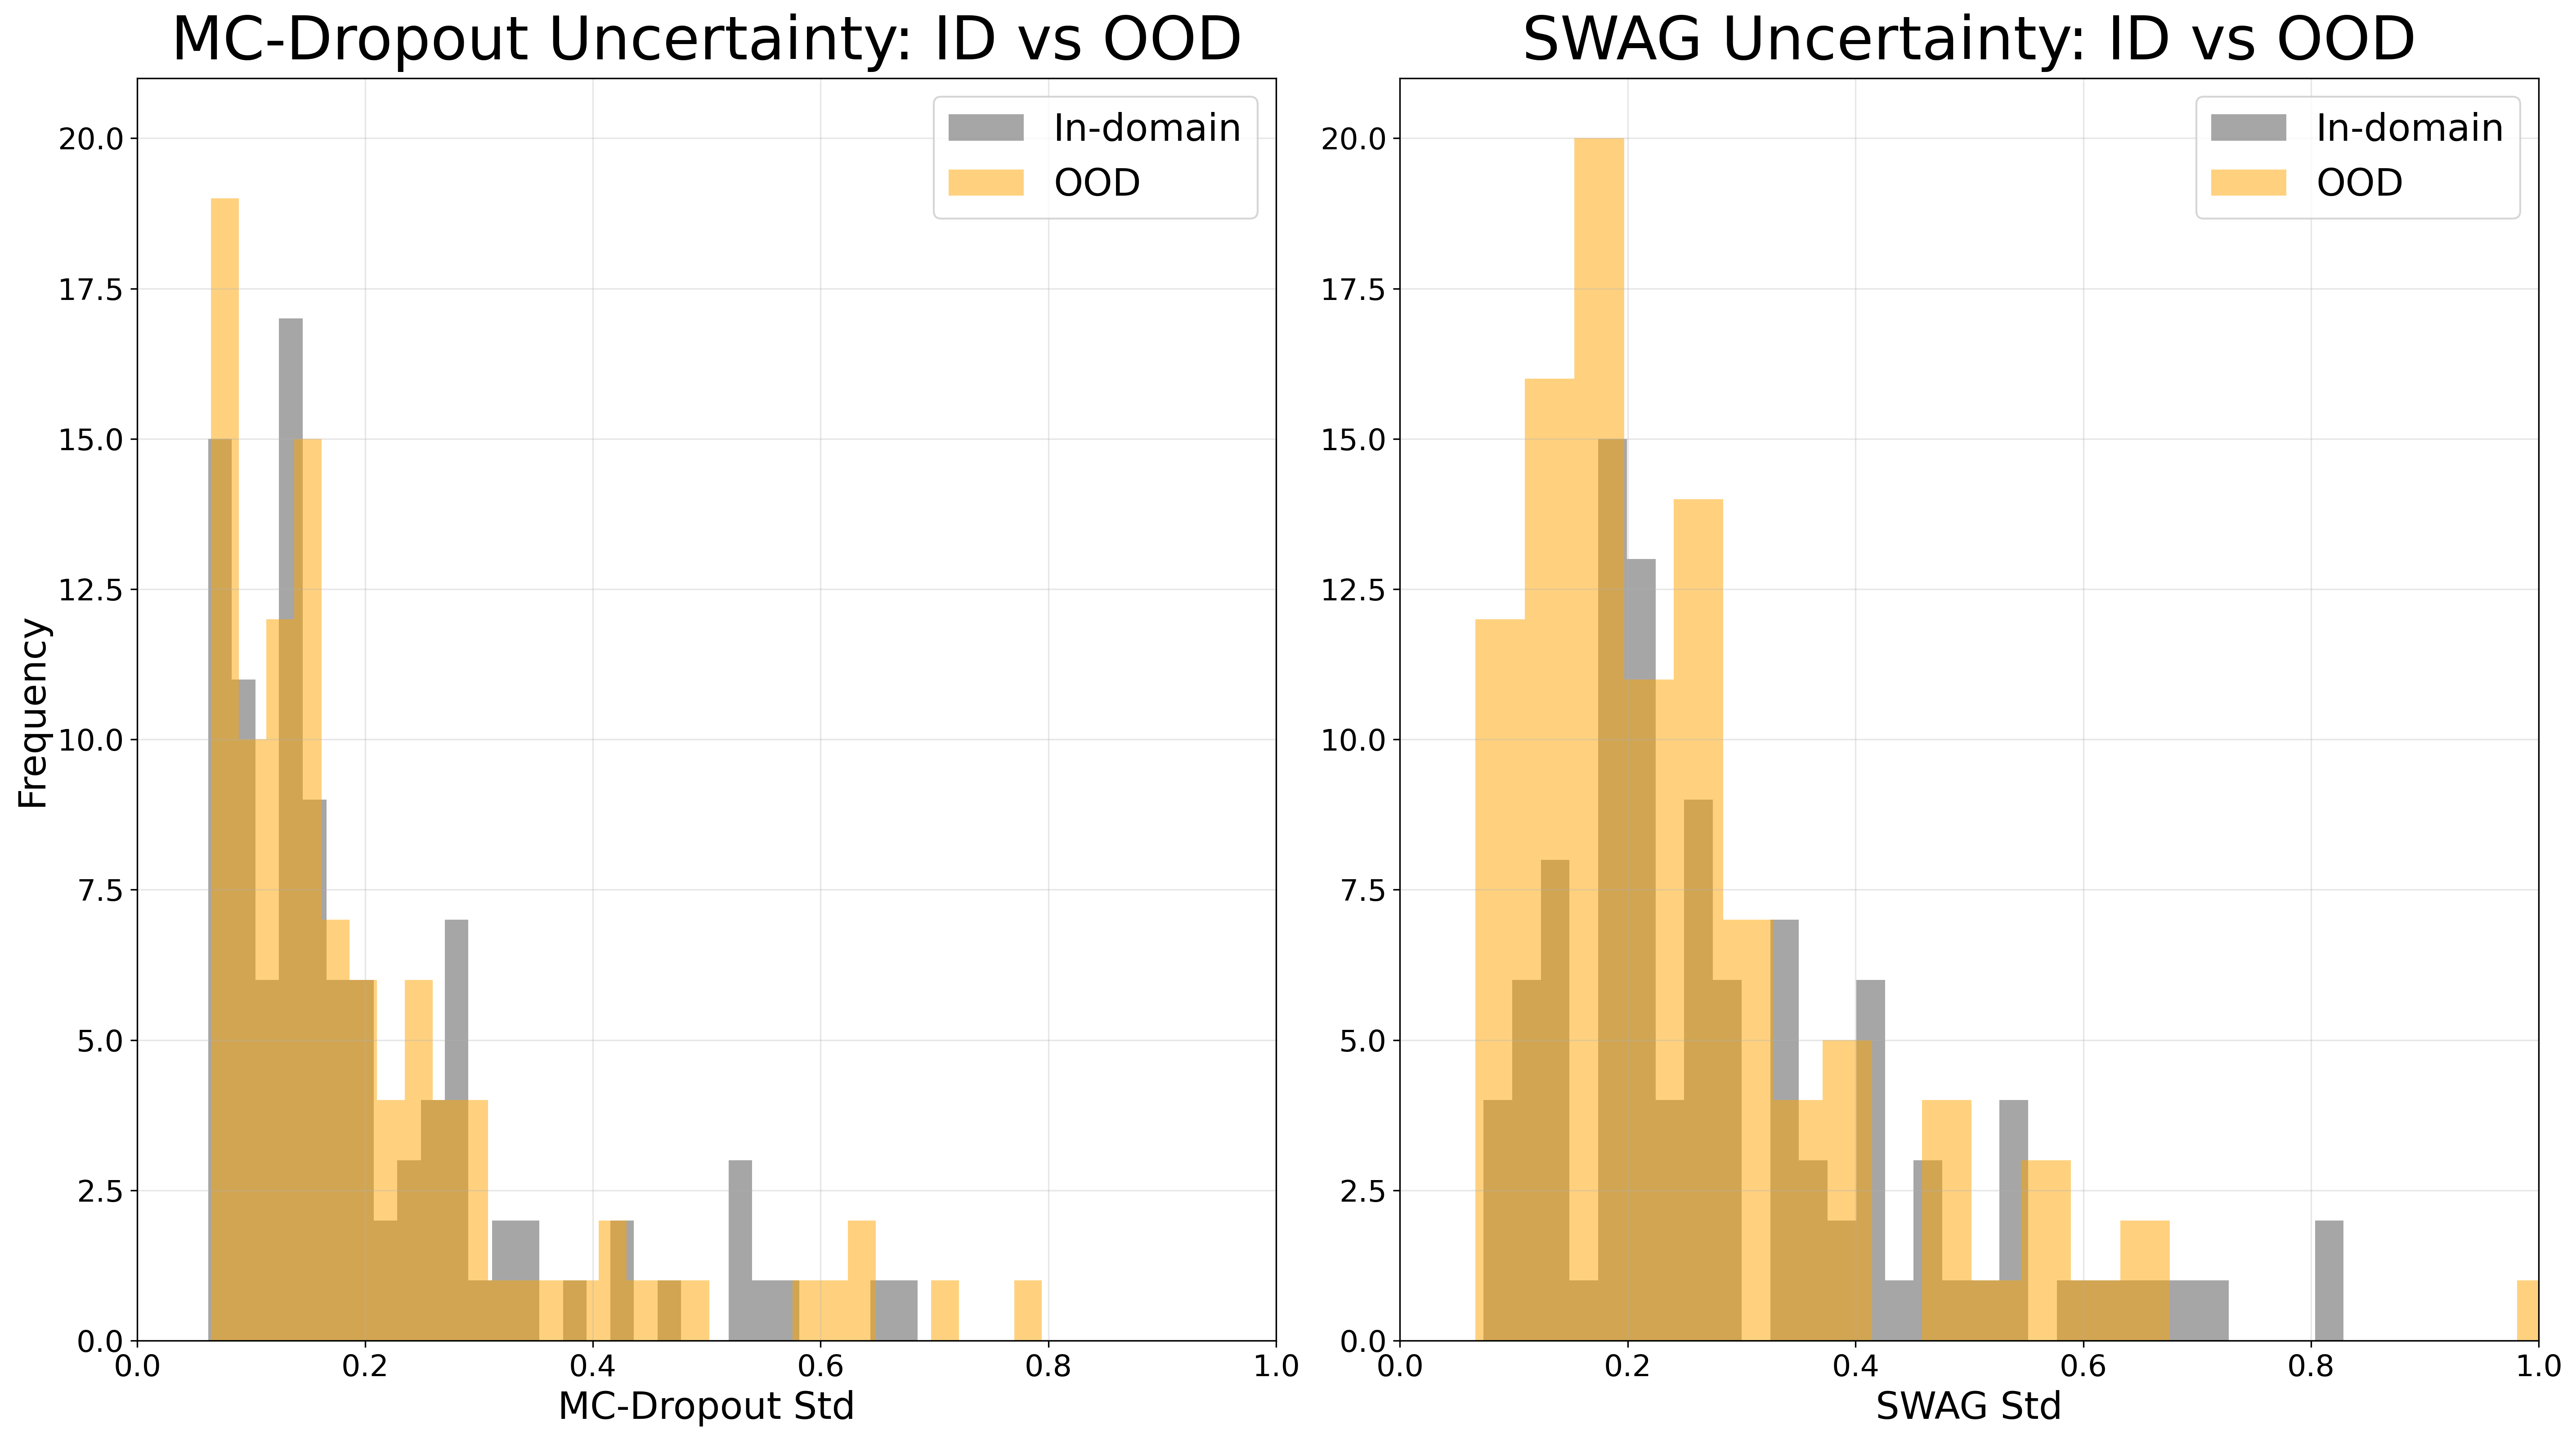
\includegraphics[width=0.9\linewidth]{plots/bh_ood_comp.png}
    \caption{Uncertainty comparison between in-domain and out-of-distribution (OOD) samples for MC-Dropout (left) and SWAG (right).}
    \label{fig:bh_ood_comp}
\end{figure}

\FloatBarrier

The Boston Housing evaluation demonstrates distinct characteristics between SWAG and MC-Dropout.
Both methods achieve comparable point-prediction accuracy, but SWAG exhibits superior uncertainty
calibration as evidenced by lower NLL and near-ideal PICP. Uncertainty visualization reveals SWAG's more
diverse uncertainty distribution and stronger error-uncertainty correlation. Under distribution shift,
SWAG maintains stable accuracy while appropriately inflating uncertainty, whereas MC-Dropout shows
concerning overconfidence.
